\documentclass[11pt]{article}
\usepackage{amssymb,graphicx,amsmath,mathtools,float}
\usepackage{lscape}
\usepackage[utf8]{inputenc}
\usepackage[spanish, es-tabla]{babel}

\usepackage{indentfirst}	% Tabular tras un section
\usepackage{hyperref}
\hypersetup{
	colorlinks=false,
	citecolor=black,
	filecolor=black,
	linkcolor=red,
	urlcolor=black,
	pdfborderstyle={/S/U/W 1}
}

\usepackage[svgnames]{xcolor}
\definecolor{griscaption}{RGB}{100,100,100}
\usepackage{caption}
\usepackage[font={color=griscaption},figurename=Fig.,labelfont={bf}]{caption}


\newtheorem{theorem}{Theorem}
\newtheorem{corollary}[theorem]{Corollary}
\newtheorem{lemma}[theorem]{Lemma}
\newtheorem{proposition}[theorem]{Proposition}
\newtheorem{definition}[theorem]{Definición}

\newcommand\ddfrac[2]{\frac{\displaystyle #1}{\displaystyle #2}}







\title{Determinación de Órbitas Elípticas}
\author{Simón López
\\
{\small Matemáticas e Ingeniería Informática}
\\
{\small Universidad de Granada, 18071 Granada, Spain}
\\
{\small simondelosbros@correo.ugr.es}}
\date{\today}
\setlength{\unitlength}{1cm}
\setlength{\unitlength}{1cm}


\begin{document}

\section{Estudio de la unicidad de la solución}

\subsection{\normalfont{\textit{Ecuaciones fundamentales en el método de Laplace}}}
\label{subsec:fundamental_equations}
Para terminar la explicación del método de determinación con tres observaciones, recapitulemos viendo las principales ecuaciones utilizadas para obtener la órbita del objeto observado. Las ecuaciones fundamentales serán las de \eqref{eq:fundamental_equations}, que involucrarán las coordenadas angulares $\lambda$, $\mu$, $\nu$ y sus derivadas, las cuáles conocemos su valor aproximado por \ref{subsec:primera_segunda_derivada} o \ref{subsec:series_potencias}. Por otra parte, el valor de $\rho$ y sus derivadas se obtendrá resolviendo las ecuaciones fundamentales utilizando la regla de Cramer, como vimos en anteriores apartados. Nos faltaría por calcular $\rho''$, donde el determinante para el numerador es el siguiente: 
\[
\left|
\begin{array}{ccc}
-k^2X & 2\lambda' & \lambda''+\frac{k^2\lambda}{r^3}\\
-k^2Y & 2\mu' & \mu''+\frac{k^2\mu}{r^3}\\
-k^2Z & 2\nu' & \nu''+\frac{k^2\nu}{r^3}
\end{array}
\right|
=-2k^2
\left|
\begin{array}{ccc}
X & \lambda' & \lambda''\\
Y & \mu' & \mu''\\
Z & \nu' & \nu''
\end{array}
\right|
-\frac{2k^4}{r^3}
\left|
\begin{array}{ccc}
X & \lambda' & \lambda\\
Y & \mu' & \mu\\
Z & \nu' & \nu
\end{array}
\right|
=
D_3-\frac{k^2D_1}{r^3}
\]

El signo negativo delante del determinante $D_1$ aparece por intercambiar la primera y la tercera columna del determinante inmediatamente anterior.\\

Así, tenemos que los valores de $\rho$ y sus derivadas pueden ser calculados mediante:
\begin{align}
\left\{
\def\arraystretch{1.5}
\begin{array}{l}
	\rho   = \ddfrac{D_1}{D}[\ddfrac{1}{R^3}-\ddfrac{1}{r^3}]\\
	\rho'  = \ddfrac{D_2}{D}[\ddfrac{1}{R^3}-\ddfrac{1}{r^3}]\\
	\rho'' = \ddfrac{D_3}{D}[\ddfrac{1}{R^3}-\ddfrac{1}{r^3}]
\end{array}
\right.
\label{eq:rho_values}
\end{align}

\noindent con $D$, $D_1$ y $D_2$ definidos anteriormente.\\

Los determinantes $D$, $D_1$, $D_2$, $D_3$ están sujetos a pequeños errores dado que los valores implicados en ellos están calculados de forma aproximada, aunque dichos errores podrán ser corregidos tras calcular de forma aproximada el valor de $\rho$ y $\rho'$ con las ecuaciones superiores. Además, trabajamos bajo el supuesto de que las observaciones al objeto son realizadas desde el centro de la Tierra, y no desde un punto concreto de ella. Tras haber calculado de forma aproximada las distancias podremos corregir dichas observaciones por los efectos de la posición del observador sobre un punto en la superficie de la Tierra.\\


\subsection{\normalfont{\textit{Ecuaciones para la determinación de las distancias $r$ y $\rho$}}}
\label{subsec:distancias_r_rho}
Recordemos la imagen \ref{fig:notation} en la que mostrábamos el triángulo formado por los tres cuerpos $S$, $E$ y $C$ junto a sus distancias. Definamos $\psi$ y $\phi$, ángulos formados en $E$ y $C$ respectivamente.

\begin{figure}[H]
\centering
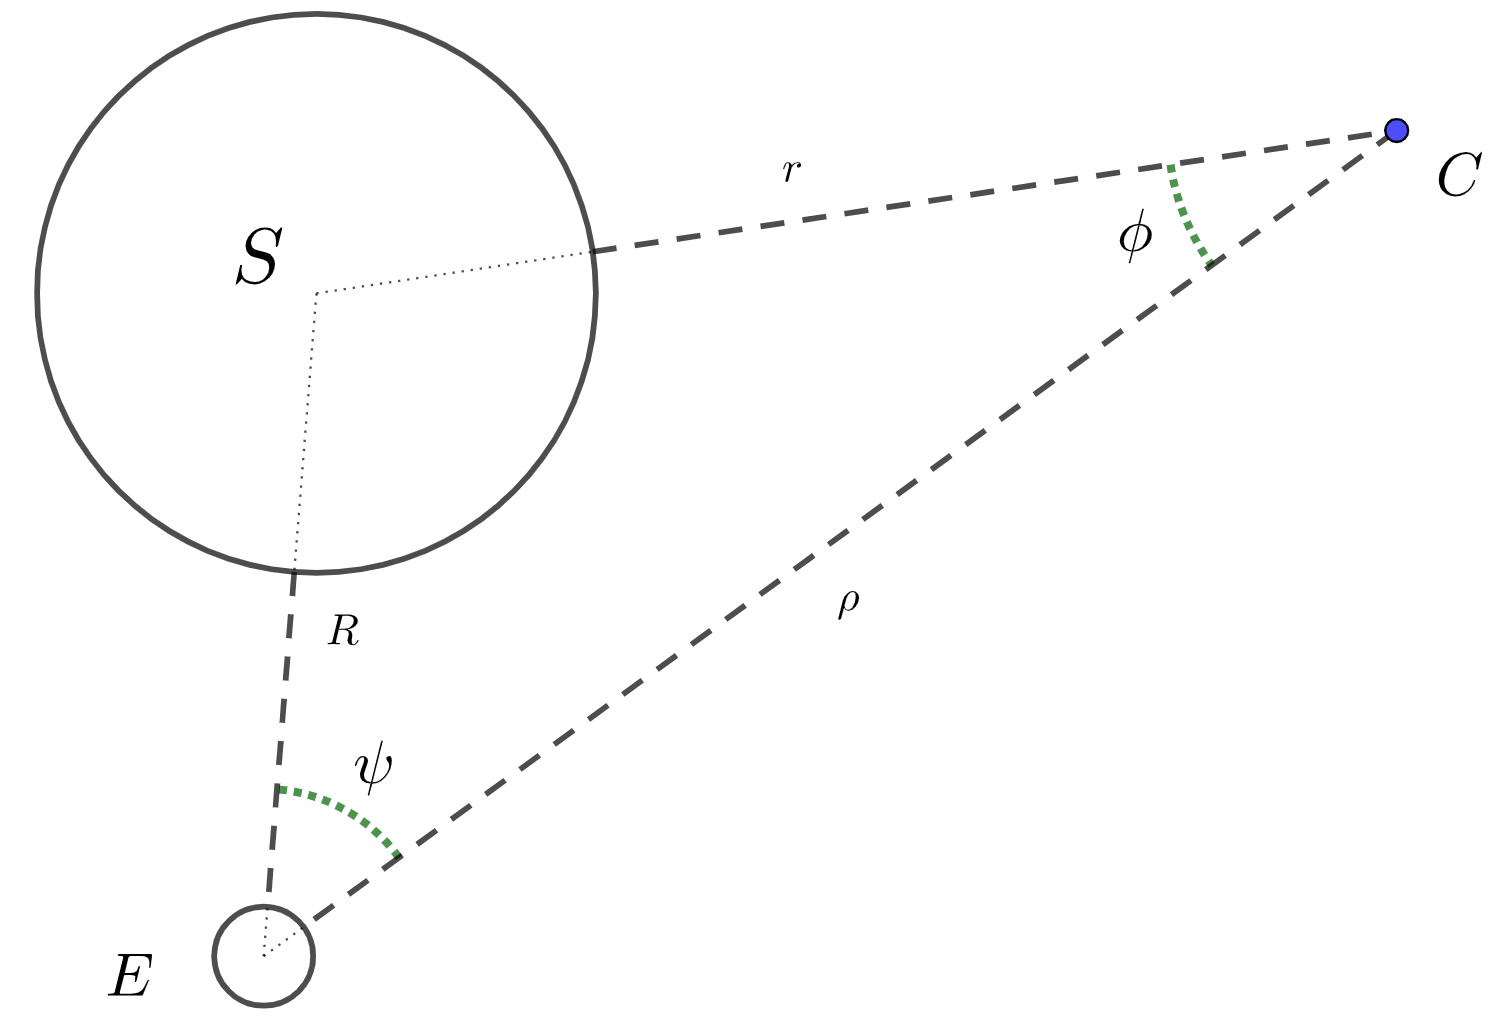
\includegraphics[scale=0.15]{images/notation_angles.png}
\caption{Triángulo formado por $S$, $E$ y $C$ junto a las distancias y ángulos generados.}
\label{fig:notation_angles}
\end{figure}

A partir de la figura superior, y junto al teorema de los senos ($\ddfrac{a}{\sin{\alpha}}=\ddfrac{b}{\sin{\beta}}=\ddfrac{c}{\sin{\gamma}}$), podemos deducir las siguientes ecuaciones:
\begin{align}
\left\{
\begin{array}{l}
	R\cos{\phi}=X\lambda+Y\mu+Z\nu\\
	\rho=R\ddfrac{\sin{(\psi+\phi)}}{\sin{\phi}}\; \; \; \; \; \cite{ASA}\\
	r=R\ddfrac{\sin{\psi}}{\sin{\phi}}
\end{array}
\right.
\label{eq:triangle_relations}
\end{align}

Sustituyendo dichas ecuaciones en la ecuación de $\rho$ en \eqref{eq:rho_values} obtenemos:
\[
R\sin{\psi}\cos{\phi}+\left(R\cos{\psi}-\ddfrac{D_1}{DR^3}\right)\sin{\phi}=\ddfrac{-D_1}{DR^3\sin^3{\psi}}\sin^4{\phi}
\]

Con el fin de simplificar esta expresión, definamos las siguientes expresiones:
\begin{align}
\left\{
\begin{array}{l}
	N\sin{m}=R\sin{\psi}\\
	N\cos{m}=R\cos{\psi}-\ddfrac{D_1}{DR^3}\\
	M=\ddfrac{-NDR^3\sin^3{\psi}}{D_1}
\end{array}
\right.
\label{eq:to_simplify}
\end{align}

El signo de $N$ será elegido de tal manera que $M$ sea positivo; fijado el signo, las dos primeras ecuaciones de \eqref{eq:to_simplify} determinarán unívocamente los valores $N$ y $m$, y la expresión que queríamos simplificar pasa a ser simplemente:
\begin{align}
\def\arraystretch{2}
\begin{array}{c}
	N\sin{m}\cos{\phi}+N\cos{m}\sin{\phi}=N\sin{(\phi+m)}=\ddfrac{N}{M}\sin^4{\phi} \Longrightarrow\\
	\Longrightarrow\sin^4{\phi}=M\sin{(\phi+m)}
\end{array}
\label{eq:phi_solution}
\end{align}

El valor para $M$ y $m$ serán conocidos cuando $M$ sea positivo. Busquemos ahora la solución de esta ecuación para $\phi$; dado que $\rho=0$ y $r=R$ es una solución al problema, podremos asegurar que $\phi=\pi-\psi$ es una solución válida, aunque no es de valor práctico dado que ésta corresponde a la posición del observador en la Tierra. Por tanto, dado que la solución ha de pertenecer al problema físico y que nos encontramos en un triángulo, podemos asegurar que:
\[
\phi<\pi-\psi
\]

Así, las soluciones de \eqref{eq:phi_solution} han de ser las intersecciones entre las curvas que definen las ecuaciones de la izquierda y de la derecha, es decir, la intersección entre:
\[
\left\{
\begin{array}{l}
y_1=\sin^4{\phi}\\
y_2=M\sin{(\phi+m)}
\end{array}
\right.
\]

Si el valor de $m$ es negativo cercano a cero y $M$ es ligeramente menor que 1, podemos ver la relación entre ambas curvas $y_1$, $y_2$ en la figura inferior:

\begin{figure}[H]
\centering
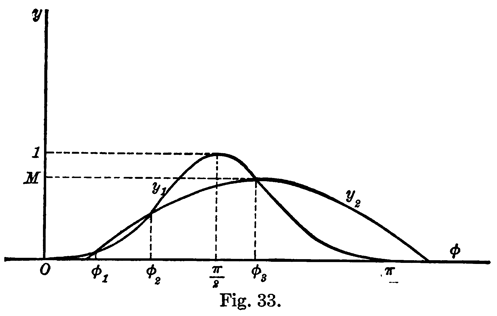
\includegraphics[scale=0.5]{images/fig_33.png}
\caption{Representación gráfica de $y_1$ e $y_2$ ($\frac{D_1}{D}>0$).}
\label{fig:y1_y2_graph_positive}
\end{figure}

En dicha imagen podemos ver que obtenemos tres intersecciones de las curvas, correspondientes cada una a una solución de \eqref{eq:phi_solution} y con $\phi_1<\phi_2<\phi_3$.\\

Discutamos ahora según el signo de $\frac{D_1}{D}$ los valores de $r$, $R$ y $m$. Comencemos considerando que $\frac{D_1}{D}$ es positivo. Es claro que $\rho$ y $r$ han de ser positivos, por lo que deducimos de la primera ecuación de \eqref{eq:rho_values} que $r$ ha de ser mayor que $R$. Por tanto, como $\psi$ ha de ser menor que 180º (pues estamos en un triángulo), utilizando las ecuaciones \eqref{eq:to_simplify} tenemos:
\[
\def\arraystretch{2}
\begin{array}{l}
M=\ddfrac{-NDR^3\sin^3{\psi}}{D_1}>0 \Longrightarrow N<0 \\
R\sin{\psi}>0 \Longrightarrow N\sin{m}>0 \Longrightarrow \sin{m}<0 \Longrightarrow m\in(\pi,2\pi)
\end{array}
\]

Por tanto, $N$ es negativo y $m$ estará en el tercer o cuarto cuadrante.\\

Si $m$ está en el cuarto cuadrante, la rama ascendente de la curva $y_2$ atraviesa el eje de abscisas $\phi$ en el primer cuadrante y, si $M<1$, las relaciones entre las dos curvas serán las que podemos ver en la figura \ref{fig:y1_y2_graph_positive}. Si el valor de $m$ es cercano a 180º tendremos tres soluciones disponibles $\phi_1$, $\phi_2$, $\phi_3$, una de las cuales corresponderá al observador ($\phi_i=\pi-\psi$). Discutamos según cuál de las tres soluciones toma este valor:
\begin{itemize}
\item Si $\phi_3=\pi-\psi$, las otras dos soluciones cumplirán todas las condiciones del problema, no pudiendo determinar cuál de las dos pertenece a la órbita real del cuerpo observado (siempre que no tengamos información adicional). Pero, podría darse el caso de que en estas condiciones los valores de $r$ y $\rho$ proporcionados por la solución $\phi_1$ fueran demasiado grandes como para que el objeto fuera visible para el observador, llegando así a la conclusión de que $\phi_2$, el cuál proporcionaría un $r$ más pequeño, pertenecería al problema físico.
\item Si $\phi_2=\pi-\psi$, se sigue del hecho de que $\phi<\pi-\psi$ que la solución ha de ser $\phi_1$.
\item Si $\phi_1=\pi-\psi$, entonces el problema no tendría solución dado que cualquiera de las otras dos soluciones sería mayor que $\pi-\psi$.
\end{itemize} 

A medida que la rama ascendente de la curva $y_2$ se mueve hacia la derecha, es decir, fijando $M$ y haciendo crecer $\phi_3$, las soluciones $\phi_1$ y $\phi_2$ tienden a coincidir, y en estas condiciones, que corresponderían a $m$ lejos de 180º en el tercer o cuarto cuadrante, el problema no tendría solución. Por tanto:
\begin{quote}
\textit{Si $\frac{D_1}{D}>0$, la distancia $r$ es mayor que $R$, el ángulo $m$ estará en el cuarto cuadrante y disponemos de dos o tres soluciones del problema físico en función de que $\phi_2$ o $\phi_3$ sea igual a $\pi-\psi$.}\\
\end{quote}

Veamos ahora el caso contrario. 

\begin{figure}[H]
\centering
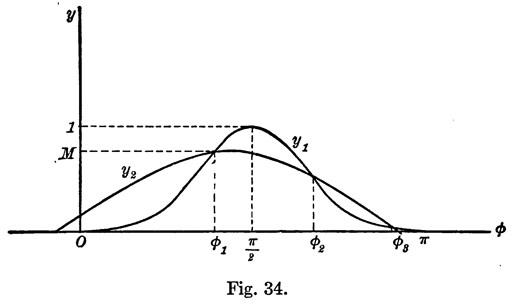
\includegraphics[scale=0.55]{images/fig_34.png}
\caption{Representación gráfica de $y_1$ e $y_2$ ($\frac{D_1}{D}<0$).}
\label{fig:y1_y2_graph_negative}
\end{figure}

Supongamos que $\frac{D_1}{D}$ es negativo, de tal manera que, procediendo como en el caso positivo, llegamos a que $r<R$ y que $m$ está en el primer o segundo cuadrante. Si $m$ está en el primer cuadrante, la rama descendente de la curva $y_2$ atraviesa el eje de abscisas $\phi$ en el segundo cuadrante, y para un $m$ pequeño y $M<1$, las relaciones entre las dos curvas serán las que podemos ver en la gráfica \ref{fig:y1_y2_graph_negative}. En este caso, la solución será única o doble en función de que $\phi_2$ o $\phi_3$ valgan $\pi-\psi$. Por último, si $m$ estuviera en el segundo cuadrante, la parte descendente de $y_2$ cortaría el eje de abscisas en el primer cuadrante, por lo que $\phi_2$ y $\phi_3$ no serían reales y el problema no tendría solución. Así, tenemos que:
\begin{quote}
\textit{Si $\frac{D_1}{D}<0$, la distancia $r$ es menor que $R$, el ángulo $m$ estará en el primer cuadrante y disponemos de dos o tres soluciones del problema físico en función de que $\phi_2$ o $\phi_3$ sea igual a $\pi-\psi$.}\\
\end{quote}



\subsection{\normalfont{\textit{Unicidad de la solución}}}
\label{subsec:unicidad}
Tal y como hemos visto en la sección anterior, la solución del problema físico será única si $\phi_2=\pi-\psi$, independientemente del signo de $\frac{D_1}{D}$; en otro caso, la solución será doble o no existirá. Sea $\varepsilon>0$ un valor pequeño y supongamos que $\phi=\pi-\psi+\varepsilon$. Entonces, si $\frac{D_1}{D}$ es positivo, podemos ver en la gráfica \ref{fig:y1_y2_graph_positive} que la diferencia $y_1-y_2$ es positiva cuando $\phi=\phi_2+\varepsilon$; y si $\frac{D_1}{D}$ es negativo, podemos ver en la gráfica \ref{fig:y1_y2_graph_negative} que $y_1-y_2$ es negativo cuando $\phi=\phi_2+\varepsilon$.\\

Sabemos que las funciones $y_1$ e $y_2$ son analíticas, y que la suma, el producto y la composición de funciones analíticas es analítica. Por tanto, $y_1-y_2$ es analítica y podremos expandirla como serie de potencias en $\varepsilon$ cuando $\phi=\pi-\psi+\varepsilon$. Así, tenemos la siguiente expresión:
\begin{align}
\begin{array}{l}
y_1-y_2=[\sin^4{(\pi-\psi)}-M\sin{(\pi-\psi+m)}]+\\+[4\sin^3{(\pi-\psi)}\cos{(\pi-\psi)}-M\cos{(\pi-\psi+m)}]\epsilon+...
\end{array}
\label{eq:y1_y2_serie}
\end{align}

\noindent donde hemos tomando $\varepsilon_0=0$ dado que $\phi=\pi-\psi$ es una solución del problema. Pasemos a simplificar esta expresión y reducir el coeficiente de $\varepsilon$ utilizando las ecuaciones \eqref{eq:to_simplify} y \eqref{eq:phi_solution}:
\[
\def\arraystretch{2}
\begin{array}{ll}
& [\sin^4{(\pi-\psi)}-\sin^4{(\pi-\psi)}]+[-4\sin^3{(\pi-\psi)}\cos{\psi}+M\cos{(-\psi+m)}]=\\
= & 0 + \left[\ddfrac{4MD_1}{NDR^3}\cos{\psi}+M(\cos{\psi}\cos{m}+\sin{\psi}\sin{m})\right]=\\
= & \ddfrac{4MD_1}{NDR^3}\cos{\psi}+M\left(\ddfrac{R\cos^2{\psi}}{N}-\ddfrac{D_1\cos{\psi}}{NDR^3}+\ddfrac{R\sin^2{\psi}}{N}\right)=\\
= & \ddfrac{4MD_1}{NDR^3}\cos{\psi}-\ddfrac{MD_1}{NDR^3}\cos{\psi}+\ddfrac{MR}{N}(\cos^2{\psi}+\sin^2{\psi})=\\
= & \ddfrac{MR}{N}\left(1+\ddfrac{3D_1}{DR^4}\cos{\psi}\right)
\end{array}
\]

\vspace{0.4cm}

Por tanto, la serie pasa a ser:
\begin{align}
y_1-y_2=\ddfrac{MR}{N}\left(1+\ddfrac{3D_1}{DR^4}\cos{\psi}\right)\varepsilon+...
\label{eq:y1_y2_serie2}
\end{align}

Así, conociendo que $MR>0$, llegamos a la conclusión de que la condición para que el problema físico tenga solución única es:
\begin{align}
\left\{
\def\arraystretch{2}
\begin{array}{l}
	\ddfrac{1}{N}\left[1+\ddfrac{3D_1}{DR^4}\cos{\psi}\right]>0 \; \; \; \; \text{si} \; \; \; \; \ddfrac{D_1}{D}>0\\
	\ddfrac{1}{N}\left[1+\ddfrac{3D_1}{DR^4}\cos{\psi}\right]<0 \; \; \; \; \text{si} \; \; \; \; \ddfrac{D_1}{D}<0
\end{array}
\right.
\label{eq:condicion_unicidad}
\end{align}

Dado que todos los valores de estas ecuaciones están dados por simples observaciones, no será necesario resolver la ecuación \eqref{eq:phi_solution} para determinar la unicidad de la solución.








\newpage

\begin{thebibliography}{99}
\bibitem{moulton} \textsc{Forest Ray Moulton}, \textsc{An Introduction to Celestial Mechanics}, \textit{second edition}.

\bibitem{ortega} \textsc{R. Ortega, A.J. Ureña}, \textsc{Introducción a la Mecánica Celeste}.

\bibitem{right_ascension_declination} \textsc{Sky \& Telescope}, \textsc{Right Ascension and Declination: Celestial Coordinates For Beginners}, \url{https://skyandtelescope.org/astronomy-resources/right-ascension-declination-celestial-coordinates/}

\bibitem{ASA} \textsc{Solution of triangles}, \url{https://en.wikipedia.org/wiki/Solution_of_triangles#A_side_and_two_adjacent_angles_given_(ASA)}

\end{thebibliography}

\end{document}
